% \iffalse meta-comment
% !TEX program  = LuaLaTeX
%
% husttrans.dtx
%
% Copyright (C) 2013-2014 by Xu Cheng <xucheng@me.com>
%               2014-2016 by hust-latex <https://github.com/hust-latex>
%
% This work may be distributed and/or modified under the
% conditions of the LaTeX Project Public License, either version 1.3
% of this license or (at your option) any later version.
% The latest version of this license is in
%   http://www.latex-project.org/lppl.txt
% and version 1.3 or later is part of all distributions of LaTeX
% version 2005/12/01 or later.
%
% This work has the LPPL maintenance status `maintained'.
%
% The Current Maintainer of this work is hust-latex Organization.
%
% This work consists of the files husttrans.dtx,
% husttrans.ins and the derived file husttrans.cls
% along with its document and example files.
%
%
% \fi
%
% \iffalse
%<*driver>
\ProvidesFile{husttrans.dtx}
%</driver>
%<class>\NeedsTeXFormat{LaTeX2e}[1999/12/01]
%<class>\ProvidesClass{husttrans}
%<*class>
[2017/02/21 v1.3 A Translation Template for Huazhong University of Science and Technology]
%</class>
%
%<*driver>
\documentclass[12pt,a4paper,numbered,full]{l3doc}

\usepackage{fontspec}
\setmainfont[Ligatures={Common,TeX}]{Tex Gyre Pagella}
\setsansfont[Ligatures={Common,TeX}]{Droid Sans}
\setmonofont{CMU Typewriter Text}
\defaultfontfeatures{Mapping=tex-text,Scale=MatchLowercase}

\usepackage{luatexja-fontspec}
\setmainjfont[BoldFont={AdobeHeitiStd-Regular},ItalicFont={AdobeKaitiStd-Regular}]{AdobeSongStd-Light}
\setsansjfont{AdobeKaitiStd-Regular}
\defaultjfontfeatures{JFM=kaiming}
\newjfontfamily\KAI{AdobeKaitiStd-Regular}
\newjfontfamily\FANGSONG{AdobeFangsongStd-Regular}

\linespread{1.2}\selectfont

\usepackage[top=1.2in,bottom=1.2in,left=1.5in,right=1in]{geometry}
\pagewidth=\paperwidth
\pageheight=\paperheight

\usepackage{color}
\usepackage[table]{xcolor}

\definecolor{hyperreflinkred}{RGB}{128,23,31}
\hypersetup{
  unicode,
  bookmarksnumbered=true,
  bookmarksopen=true,
  bookmarksopenlevel=0,
  breaklinks=true,
  colorlinks=true,
  allcolors=hyperreflinkred,
  linktoc=page,
  plainpages=false,
  pdfpagelabels=true,
  pdfstartview={XYZ null null 1}
}
\usepackage{indentfirst}
\setlength{\parindent}{2em}

\usepackage{titlesec,titletoc}
\usepackage[titles]{tocloft}
\setcounter{tocdepth}{2}
\setcounter{secnumdepth}{3}

\usepackage{enumitem}
\setlist{noitemsep,partopsep=0pt,topsep=.8ex}
\setlist[1]{labelindent=\parindent}
\setlist[enumerate,1]{label=\arabic*.,ref=\arabic*}
\setlist[enumerate,2]{label*=\arabic*,ref=\theenumi.\arabic*}
\setlist[enumerate,3]{label=\emph{\alph*}),ref=\theenumii\emph{\alph*}}

\usepackage{listings}
\definecolor{lstgreen}{rgb}{0,0.6,0}
\definecolor{lstgray}{rgb}{0.5,0.5,0.5}
\definecolor{lstmauve}{rgb}{0.58,0,0.82}
\lstset{
  basicstyle=\footnotesize\ttfamily\FANGSONG,
  keywordstyle=\color{blue}\bfseries,
  commentstyle=\color{lstgreen}\itshape\KAI,
  stringstyle=\color{lstmauve},
  showspaces=false,
  showstringspaces=false,
  showtabs=false,
  numbers=left,
  numberstyle=\tiny\color{lstgray},
  frame=lines,
  rulecolor=\color{black},
  breaklines=true
}

\AtBeginEnvironment{verbatim}{\small}
\let\AltMacroFont\MacroFont

\usepackage{metalogo}
\usepackage{notes}
\usepackage{tabularx}

\newcommand{\tabincell}[2]{\begin{tabular}{@{}#1@{}}#2\end{tabular}}

\renewcommand{\cftsecleader}{\cftdotfill{\cftdotsep}}
\setlength{\cftsecindent}{2em}
\setlength{\cftsubsecindent}{4em}
\makeatletter
\newskip\HUST@oldcftbeforepartskip
\HUST@oldcftbeforepartskip=\cftbeforepartskip
\newskip\HUST@oldcftbeforesecskip
\HUST@oldcftbeforesecskip=\cftbeforesecskip
\let\HUST@oldl@part\l@part
\let\HUST@oldl@section\l@section
\let\HUST@oldl@subsection\l@subsection
\def\l@part#1#2{\HUST@oldl@part{#1}{#2}\cftbeforepartskip=3pt}
\def\l@section#1#2{\HUST@oldl@section{#1}{#2}\cftbeforepartskip=\HUST@oldcftbeforepartskip\cftbeforesecskip=3pt}
\def\l@subsection#1#2{\HUST@oldl@subsection{#1}{#2}\cftbeforesecskip=\HUST@oldcftbeforesecskip}
\makeatother

\titleformat{\part}
  {
    \bfseries
    \centering
    \fontsize{18pt}{23.4pt}\selectfont
  }
  {\thepart}
  {1em}
  {}
\let\oldpart\part
\def\part#1{\newpage\oldpart{#1}}

\def\orvar{\textnormal{|}}

\IndexPrologue
 {
  \part{Index}
  The~italic~numbers~denote~the~pages~where~the~
  corresponding~entry~is~described,~
  numbers~underlined~point~to~the~definition,~
  all~others~indicate~the~places~where~it~is~used.
 }

\GlossaryPrologue
 {
  \part{Change History}
 }

\EnableCrossrefs
\CodelineIndex
\RecordChanges

\def\email#1{
  \href{mailto:#1}{\texttt{#1}}
}

\usepackage{xparse}
\ExplSyntaxOn
\DeclareDocumentCommand\pkgurl{o m}
{
    \IfNoValueTF{#1}
    {
        \href
        {
        http://mirrors.ctan.org/help/Catalogue/entries/
        \str_fold_case:n {#2} .html
        }
        { \textsf{#2} }
    }
    {
        \href
        {
        http://mirrors.ctan.org/help/Catalogue/entries/
        \str_fold_case:n {#1} .html
        }
        { \textsf{#2} }
    }
}
\ExplSyntaxOff

\begin{document}
\DocInput{husttrans.dtx}
\end{document}
%</driver>
% \fi
%
% \CheckSum{782}
%
% \iffalse
%<*!(example-bib)>
% \fi
%% \CharacterTable
%% {Upper-case    \A\B\C\D\E\F\G\H\I\J\K\L\M\N\O\P\Q\R\S\T\U\V\W\X\Y\Z
%%  Lower-case    \a\b\c\d\e\f\g\h\i\j\k\l\m\n\o\p\q\r\s\t\u\v\w\x\y\z
%%  Digits        \0\1\2\3\4\5\6\7\8\9
%%  Exclamation   \!     Double quote  \"     Hash (number) \#
%%  Dollar        \$     Percent       \%     Ampersand     \&
%%  Acute accent  \'     Left paren    \(     Right paren   \)
%%  Asterisk      \*     Plus          \+     Comma         \,
%%  Minus         \-     Point         \.     Solidus       \/
%%  Colon         \:     Semicolon     \;     Less than     \<
%%  Equals        \=     Greater than  \>     Question mark \?
%%  Commercial at \@     Left bracket  \[     Backslash     \\
%%  Right bracket \]     Circumflex    \^     Underscore    \_
%%  Grave accent  \`     Left brace    \{     Vertical bar  \|
%%  Right brace   \}     Tilde         \~}
% \iffalse
%</!(example-bib)>
% \fi
%
% \changes{v1.0}{2014/03/01}{Initial version}
% \changes{v1.1}{2016/06/01}{Fix for TeXLive 2016. Remove \texttt{interfaces} and other problematic package}
% \changes{v1.2}{2016/07/05}{Fix for \XeLaTeX}
% \changes{v1.3}{2017/02/21}{Fix page style}
%
% \GetFileInfo{husttrans.dtx}

%
% \DoNotIndex{\#,\$,\%,\&,\@,\\,\{,\},\^,\_,\~,\ ,\,}
% \DoNotIndex{\def,\if,\else,\fi,\gdef,\long,\let}
% \DoNotIndex{\@ne,\@nil}
% \DoNotIndex{\begingroup,\endgroup,\advance}
% \DoNotIndex{\newcommand,\renewcommand}
% \DoNotIndex{\newenvironment,\renewenvironment}
% \DoNotIndex{\RequirePackage}
%
% \title{A Translation Template for Huazhong University of Science and Technology: the \textsf{husttrans} class
% \thanks{This document corresponds to \textsf{husttrans.cls}~\fileversion, dated \filedate.}}
% \author{Xu Cheng \\ \email{xucheng@me.com}}
% \date{\today}
%
% \begingroup
% \hypersetup{allcolors=black}
% \maketitle
% \endgroup
% \tableofcontents
%
% \part{Introduction}
%
% This is a translation template for \href{http://www.hust.edu.cn/}{Huazhong University of Science \& Technology}. This template is distributed in the hope that it will be useful, but WITHOUT ANY WARRANTY; without even the implied warranty of MERCHANTABILITY or FITNESS FOR A PARTICULAR PURPOSE.
%
% The whole project is published under LPPL v1.3 License at \href{https://github.com/hust-latex/husttrans}{GitHub}.
%
% \part{使用说明}\label{part:使用说明}
% \section{使用必要条件}
%
% \begin{enumerate}
%     \item 安装最新版本的\href{http://www.tug.org/texlive/}{\texttt{TeXLive}}(推荐)或\href{http://miktex.org/}{\texttt{MiKTeX}}。因为未及时更新的宏包可能存在未修复的bug,请确保所有宏包都更新至最新。
%     \item 安装如下中文字体\footnote{本模板所用到的英文字体\textsf{Tex Gyre Termes},\textsf{Droid Sans}和\textsf{CMU Typewriter Text}均默认安装于\textsf{TeXLive}和\textsf{MiKTeX}中。}:
%     \begin{enumerate}[label=\emph{\alph*})]
%         \item \textsf{AdobeSongStd-Light}
%         \item \textsf{AdobeKaitiStd-Regular}
%         \item \textsf{AdobeHeitiStd-Regular}
%         \item \textsf{AdobeFangsongStd-Regular}
%     \end{enumerate}
%     \begin{informationnote}
%     如果使用\textnormal{\LuaTeX},安装字体之后需运行命令\verb+mkluatexfontdb+生成字体索引。
%     \end{informationnote}
% \end{enumerate}
%
% \section{安装}
%
% \subsection{安装到本地}
%
% 使用如下命令即可安装本模板到本地:
% \begin{verbatim}
%     make install
% \end{verbatim}
% 如需卸载,则使用如下命令:
% \begin{verbatim}
%     make uninstall
% \end{verbatim}
%
% 对于没有安装\verb+Make+的Windows系统用户,可以使用如下命令安装:
% \begin{verbatim}
%     makewin32.bat install
% \end{verbatim}
% 如需卸载,则使用如下命令:
% \begin{verbatim}
%     makewin32.bat uninstall
% \end{verbatim}
% 虽然\verb+makewin32.bat+表现与\verb+Makefile+极其相似,但是还是强烈建议你安装\verb+Make+,对于Windows用户可以在\href{http://gnuwin32.sourceforge.net/packages/make.htm}{这里}下载。
%
% \subsection{免安装使用}
%
% 如果你希望临时使用本模板,而非安装到本地供长期使用。使用如下命令解压模板文件:
% \begin{verbatim}
%     make unpack
% \end{verbatim}
% 对于没有安装\verb+Make+的Windows系统用户,则使用如下命令解压:
% \begin{verbatim}
%     makewin32.bat unpack
% \end{verbatim}
%
% 再将\verb+husttrans+目录下的如下文件拷贝到你\TeX{}工程根目录下即可:
% \begin{itemize}
%     \item \verb+husttrans.cls+
% \end{itemize}
%
% \section{基本用法}
%
% \begin{importantnote}
% 本文档只能使用\textnormal{\XeLaTeX}或\textnormal{\LuaLaTeX}(推荐)编译。
% \end{importantnote}
%
% 在源文件开头处选择加载本文档类型,即可使用本模板,如下所示:
% \begin{verbatim}
%     \documentclass{husttrans}
% \end{verbatim}
%
% \subsection{基本字段设置}
%
% 模板中定义一些命令用于设置文档中的字段。
% \begin{function}{\title}
%     \begin{syntax}
%     \cs{title}\Arg{translation title}\
%     \end{syntax}
%     该命令用于设定外文翻译的标题。
% \end{function}
%
% \begin{function}{\author}
%     \begin{syntax}
%     \cs{author}\Arg{Orignial author}
%     \end{syntax}
%     该命令用于设定原文作者。
% \end{function}
%
% \begin{function}{\translator}
%     \begin{syntax}
%     \cs{translator}\Arg{Translator}
%     \end{syntax}
%     该命令用于设定翻译作者。
% \end{function}
%
% \begin{function}{\date}
%     \begin{syntax}
%     \cs{date}\Arg{Year}\Arg{Month}\Arg{Day}
%     \end{syntax}
%     该命令用于设定日期。如果不设定,则会选择当前编译日期。
% \end{function}
%
% \begin{function}{\supervisor}
%     \begin{syntax}
%     \cs{supervisor}\Arg{supervisor}
%     \end{syntax}
%     该命令用于设定指导老师名(含职称)。
% \end{function}
%
% \subsection{其它基本命令}
%
% 下面来介绍其它基本命令。
%
% \begin{function}{\frontmatter,\mainmatter,\backmatter}
%     这一组命令用于设定译文的状态、改变样式,其具体使用见\nameref{sec:简单示例}。\verb+\frontmatter+用在文档最开始,表明文档的前言部分(如封面,目录等)的开始。\verb+\mainmatter+表示译文正文的开始。\verb+\backmatter+表示译文正文的结束。
% \end{function}
%
% \begin{function}{\maketitle,\makecover}
%     \verb+\maketitle+和\verb+\makecover+作用相同,用于生成封面。
% \end{function}
%
% \begin{function}{\tableofcontents}
%     用于生成目录。
% \end{function}
%
% \begin{function}{\dateformat}
%     用于打印日期。
% \end{function}
%
% \begin{function}{\bibliography}
%     \begin{syntax}
%     \cs{bibliography}\Arg{.bib file}
%     \end{syntax}
%     用于生成参考文献。
% \end{function}
%
% \vskip 1ex\DescribeEnv{appendix}
%     \verb+appendix+环境用于附录环境。你可以将附录置于\verb+appendix+环境中,如:
%     \begin{verbatim}
%     \begin{appendix}
%         <content>
%     \end{appendix}
%     \end{verbatim}
% \begin{function}{\appendix}
%     或者使用\verb+\appendix+代表后文均为附录,如:
%     \begin{verbatim}
%     \appendix
%     <content>
%     \end{verbatim}
% \end{function}
%
% \begin{function}{\listoffigures,\listoftables}
%     这两个命令分别用于生成图片和表格索引,可以根据要求在前言中或附录中使用。
% \end{function}
%
% \begin{function}{\TurnOffTabFontSetting,\TurnOnTabFontSetting}
%     因为模板中设定了表格的行距和字号,使得使用中无法临时自定义表格的行距和字号。故提供两个命令用于关闭和开启默认表格的行距和字号设置。比如你如果需要输出一个自己定义字号的表格,可以使用如下示例:
%     \begin{verbatim}
%     \begingroup
%     \TurnOffTabFontSetting
%     \footnotesize % 设置字号
%     \begin{tabular}{...}
%         <content>
%     \end{tabular}
%     \TurnOnTabFontSetting
%     \endgroup
%     \end{verbatim}
% \end{function}
%
% \begin{function}{\email}
%     \begin{syntax}
%     \cs{email}\Arg{Email Address}
%     \end{syntax}
%     用于生成邮箱地址。如\verb+\email{name@example.com}+会生成如下效果的地址:\email{name@example.com}。
% \end{function}
%
% \section{简单示例}\label{sec:简单示例}
% 如下为一个使用本模板的简单示例。更完整的例子请见\texttt{husttrans-example.tex}文件,其效果见\href{https://github.com/hust-latex/husttrans/raw/master/husttrans/husttrans-example.pdf}{\texttt{husttrans-example.pdf}}。
%
% \iffalse
%<*driver>
% \fi
\begin{lstlisting}[language={[LaTeX]TeX}]
\documentlcass{husttrans}
\title{原文标题}
\author{原文作者}
\translator{翻译作者}
\supervisor{指导老师}
\date{2014}{3}{1}

\begin{document}

\frontmatter
\maketitle
\tableofcontents
\listoffigures
\listoftables
\mainmatter

%% 正文

\backmatter
\bibliography{参考文献.bib文件}
\appendix
%% 附录剩余部分
\end{document}
\end{lstlisting}
% \iffalse
%</driver>
% \fi
%
%
% \section{预设宏包介绍}
%
% 本模板中预设了一些宏包,下面对其进行简单介绍。
%
% \begin{itemize}
%     \item \pkgurl{algorithm2e} 算法环境。
%     \item \pkgurl{enumitem} 自定义列表环境的式样。
%     \item \pkgurl{fancynum} 用于将大数每三位断开。
%     \item \pkgurl{listings} 代码环境。如需更好的代码高亮可以使用\pkgurl{minted}宏包。
%     \item \pkgurl{longtable} 跨页的超长表格环境。
%     \item \pkgurl{ltxtable} \textsf{longtable}环境和\textsf{tabularx}环境的合并。
%     \item \pkgurl{multirow} 用于表格中合并行。
%     \item \pkgurl{overpic} 用于在图片上层叠其他内容。
%     \item \pkgurl{tabularx} 扩展到表格环境。
%     \item \pkgurl{zhnumber} 用于生成中文数字。
% \end{itemize}
%
% \section{高级设置}
%
% \subsection{切换字体}
%
% 模板正文字体为宋体(\textsf{AdobeSongStd-Light}),同时我们提供如下命令切换中文字体:
%
% \begin{function}{\HEI,\hei}
%     \begin{syntax}
%     \{\cs{HEI} \meta{content}\}
%     \cs{hei}\Arg{content}
%     \end{syntax}
%     切换字体为黑体(\textsf{AdobeHeitiStd-Regular})。
% \end{function}
%
% \begin{function}{\KAI,\kai}
%     \begin{syntax}
%     \{\cs{KAI} \meta{content}\}
%     \cs{kai}\Arg{content}
%     \end{syntax}
%     切换字体为楷体(\textsf{AdobeKaitiStd-Regular})。
% \end{function}
%
% \begin{function}{\FANGSONG,\fangsong}
%     \begin{syntax}
%     \{\cs{FANGSONG} \meta{content}\}
%     \cs{fangsong}\Arg{content}
%     \end{syntax}
%     切换字体为仿宋(\textsf{AdobeFangsongStd-Regular})。
% \end{function}
%
% 如果需要加载其他字体,请参阅宏包\pkgurl{fontspec},宏包\pkgurl{xeCJK}(对于\XeLaTeX{})和宏包\pkgurl[luatexja]{luatex-ja}(对于\LuaLaTeX{})的文档。
%
% \subsection{内部字段设置}
% 本模板定义了内部字段,其具体内容见\autoref{sec:Localization}。通过更改这些字段,可以对格式进行自定义。
%
% \StopEventually{
%  \PrintIndex
%  \PrintChanges
% }
%
% \part{Implementation}\label{part:Implementation}
%
%    \begin{macrocode}
%<*class>
\RequirePackage{ifthen}
%    \end{macrocode}
%
% \section{Process Options}
% Use \pkgurl{xkeyval} to process options.
%    \begin{macrocode}
\RequirePackage{xkeyval}
%    \end{macrocode}
%
% Process options and load class |book|.
%    \begin{macrocode}
\DeclareOption*{\PassOptionsToClass{\CurrentOption}{book}}
\ProcessOptionsX
\LoadClass[12pt, a4paper, openany]{book}
%    \end{macrocode}
%
% \section{Check Engine}
% Check engine, only \XeLaTeX{} and \LuaLaTeX{} are supported.
%    \begin{macrocode}
\RequirePackage{iftex}
\ifXeTeX\else
  \ifLuaTeX\else
    \begingroup
      \errorcontextlines=-1\relax
      \newlinechar=10\relax
      \errmessage{^^J
      *******************************************************^^J
      * XeTeX or LuaTeX is required to compile this document.^^J
      * Sorry!^^J
      *******************************************************^^J
      }%
    \endgroup
  \fi
\fi
%    \end{macrocode}
%
% \section{Font Setting}
% Set font used in document. Firstly, it's English font. We use \pkgurl{fontspec} package to handle font. We choose \textsf{Tex Gyre Termes}, \textsf{Droid Sans} and \textsf{CMU Typewriter Text} as document main font, sans font and mono font.
%
% Then it's the Chinese font setting. We use \pkgurl{xecjk} package (for \XeLaTeX) or \pkgurl[luatexja]{luatex-ja} package (for \LuaLaTeX, recommend) to handle Chinese font. We will use font: \textsf{AdobeSongStd-Light}, \textsf{AdobeKaitiStd-Regular}, \textsf{AdobeHeitiStd-Regular} and \textsf{AdobeFangsongStd-Regular}.
%    \begin{macrocode}
\ifXeTeX  % XeTeX下使用fontspec + xeCJK处理字体
  % 英文字体
  \RequirePackage{fontspec}
  \RequirePackage{xunicode}
  \setmainfont[
    Ligatures={Common,TeX},
    Extension=.otf,
    UprightFont=*-regular,
    BoldFont=*-bold,
    ItalicFont=*-italic,
    BoldItalicFont=*-bolditalic]{texgyretermes}
  \setsansfont[Ligatures={Common,TeX}]{Droid Sans}
  \setmonofont{CMU Typewriter Text}
  \defaultfontfeatures{Mapping=tex-text}
  % 中文字体
  \RequirePackage[CJKmath]{xeCJK}
  \setCJKmainfont[
   BoldFont={Adobe Heiti Std},
   ItalicFont={Adobe Kaiti Std}]{Adobe Song Std}
  \setCJKsansfont{Adobe Kaiti Std}
  \setCJKmonofont{Adobe Fangsong Std}
  \xeCJKsetup{PunctStyle=kaiming}

  \newcommand\ziju[2]{{\renewcommand{\CJKglue}{\hskip #1} #2}}
%    \end{macrocode}
%
% \begin{macro}{\HEI}
%    \begin{macrocode}
  \newCJKfontfamily\HEI{Adobe Heiti Std}
%    \end{macrocode}
% \end{macro}
%
% \begin{macro}{\KAI}
%    \begin{macrocode}
  \newCJKfontfamily\KAI{Adobe Kaiti Std}
%    \end{macrocode}
% \end{macro}
%
% \begin{macro}{\FANGSONG}
%    \begin{macrocode}
  \newCJKfontfamily\FANGSONG{Adobe Fangsong Std}
%    \end{macrocode}
% \end{macro}
%
% \begin{macro}{\hei}
%    \begin{macrocode}
  \newcommand{\hei}[1]{{\HEI #1}}
%    \end{macrocode}
% \end{macro}
%
% \begin{macro}{\kai}
%    \begin{macrocode}
  \newcommand{\kai}[1]{{\KAI #1}}
%    \end{macrocode}
% \end{macro}
%
% \begin{macro}{\fangsong}
%    \begin{macrocode}
  \newcommand{\fangsong}[1]{{\FANGSONG #1}}
%    \end{macrocode}
% \end{macro}
%
%    \begin{macrocode}
\else\fi
\ifLuaTeX  % LuaTeX下使用luatex-ja处理字体 [推荐]
  \RequirePackage{luatexja-fontspec}
  % 英文字体
  \setmainfont[Ligatures={Common,TeX}]{Tex Gyre Termes}
  \setsansfont[Ligatures={Common,TeX}]{Droid Sans}
  \setmonofont{CMU Typewriter Text}
  \defaultfontfeatures{Mapping=tex-text,Scale=MatchLowercase}
  % 中文字体
  \setmainjfont[
   BoldFont={AdobeHeitiStd-Regular},
   ItalicFont={AdobeKaitiStd-Regular}]{AdobeSongStd-Light}
  \setsansjfont{AdobeKaitiStd-Regular}
  \defaultjfontfeatures{JFM=kaiming}

  \newcommand\ziju[2]{\vbox{\ltjsetparameter{kanjiskip=#1} #2}}
%    \end{macrocode}
%
% \begin{macro}{\HEI}
%    \begin{macrocode}
  \newjfontfamily\HEI{AdobeHeitiStd-Regular}
%    \end{macrocode}
% \end{macro}
%
% \begin{macro}{\KAI}
%    \begin{macrocode}
  \newjfontfamily\KAI{AdobeKaitiStd-Regular}
%    \end{macrocode}
% \end{macro}
%
% \begin{macro}{\FANGSONG}
%    \begin{macrocode}
  \newjfontfamily\FANGSONG{AdobeFangsongStd-Regular}
%    \end{macrocode}
% \end{macro}
%
% \begin{macro}{\hei}
%    \begin{macrocode}
  \newcommand{\hei}[1]{{\jfontspec{AdobeHeitiStd-Regular} #1}}
%    \end{macrocode}
% \end{macro}
%
% \begin{macro}{\kai}
%    \begin{macrocode}
  \newcommand{\kai}[1]{{\jfontspec{AdobeKaitiStd-Regular} #1}}
%    \end{macrocode}
% \end{macro}
%
% \begin{macro}{\fangsong}
%    \begin{macrocode}
  \newcommand{\fangsong}[1]{{\jfontspec{AdobeFangsongStd-Regular} #1}}
%    \end{macrocode}
% \end{macro}
%
%    \begin{macrocode}
\else\fi
%    \end{macrocode}
%
% Generate Chinese number using \pkgurl{zhnumber}.
%    \begin{macrocode}
\RequirePackage{zhnumber}
\def\CJKnumber#1{\zhnumber{#1}} % 兼容CJKnumb
%    \end{macrocode}
%
% \section{Basic Format}
% We set global line spread to 1.3.
%    \begin{macrocode}
\linespread{1.3}\selectfont
%    \end{macrocode}
%
% Use \pkgurl{geometry} package to handle paper page.
%    \begin{macrocode}
\RequirePackage{geometry}
\geometry{
  top=1.2in,
  bottom=1.2in,
  left=1in,
  right=1in,
  includefoot
}
\ifthenelse{\isundefined{\pagewidth}}{
  \pdfpagewidth=\paperwidth
  \pdfpageheight=\paperheight
}{
  \pagewidth=\paperwidth
  \pageheight=\paperheight
}
%    \end{macrocode}
%
% Indent of paragraph and skip between paragraphs.
%    \begin{macrocode}
\RequirePackage{indentfirst}
\setlength{\parindent}{2em}
\setlength{\parskip}{0pt plus 2pt minus 1pt}
%    \end{macrocode}
%
% Packages to handle color.
%    \begin{macrocode}
\RequirePackage{color}
\RequirePackage[table]{xcolor}
%    \end{macrocode}
%
% Use \pkgurl{hyperref} package to generate cross-reference link.
%    \begin{macrocode}
\RequirePackage[unicode]{hyperref}
\hypersetup{
  bookmarksnumbered=true,
  bookmarksopen=true,
  bookmarksopenlevel=1,
  breaklinks=true,
  colorlinks=true,
  allcolors=black,
  linktoc=all,
  plainpages=false,
  pdfpagelabels=true,
  pdfstartview={XYZ null null 1},
  pdfinfo={Template.Info={husttrans.cls v1.0 2014/03/01, Copyright (C) 2013-2014 by Xu Cheng 2014 by hust-latex, https://github.com/hust-latex/husttrans}}
}
%    \end{macrocode}
%
% \section{Load Packages}
% Load packages for math.
%    \begin{macrocode}
\RequirePackage{amsmath,amssymb,amsfonts}
\RequirePackage[amsmath,amsthm,thmmarks,hyperref,thref]{ntheorem}
\RequirePackage{fancynum}
\setfnumgsym{\,}
\RequirePackage[lined,boxed,linesnumbered,ruled,vlined,algochapter]{algorithm2e}
%    \end{macrocode}
%
% Load packages for picture.
%    \begin{macrocode}
\RequirePackage{overpic}
\RequirePackage{graphicx,caption,subcaption}
%    \end{macrocode}
%
% Load packages for table.
%    \begin{macrocode}
\RequirePackage{array}
\RequirePackage{multirow,tabularx,ltxtable}
%    \end{macrocode}
%
% Load package for code highlight. Here we use \pkgurl{listings} to highlight the code. But if you need more features, use \pkgurl{minted}.
%    \begin{macrocode}
\RequirePackage{listings}
%    \end{macrocode}
%
% Load package for bibliography cite style.
%    \begin{macrocode}
\RequirePackage[numbers,square,comma,super,sort&compress]{natbib}
%    \end{macrocode}
%
% Other packages for style setting.
%    \begin{macrocode}
\RequirePackage{titlesec}
\RequirePackage{titletoc}
\RequirePackage{tocvsec2}
\RequirePackage[inline]{enumitem}
\RequirePackage{fancyhdr}
\RequirePackage{afterpage}
\RequirePackage{datenumber}
\RequirePackage{etoolbox}
\RequirePackage{appendix}
\RequirePackage[titles]{tocloft}
\RequirePackage{xstring}
\RequirePackage{perpage}
%    \end{macrocode}
%
% \section{Variables Setting}
% \begin{macro}{\title}
% Commands to set the title.
%    \begin{macrocode}
\def\title#1{\gdef\HUST@zhtitle{#1}\hypersetup{pdftitle={#1}}}
\title{}
%    \end{macrocode}
% \end{macro}
%
% \begin{macro}{\author}
% Commands to set the author.
%    \begin{macrocode}
\def\author#1{\gdef\HUST@zhauthor{#1}}
\author{}
%    \end{macrocode}
% \end{macro}
%
% \begin{macro}{\translator}
% Commands to set the translator.
%    \begin{macrocode}
\def\translator#1{\gdef\HUST@zhtranslator{#1}\hypersetup{pdfauthor={#1}}}
\translator{}
%    \end{macrocode}
% \end{macro}

%
% \begin{macro}{\date,\dateformat}
% A command to set the date and several commands to display date.
%    \begin{macrocode}
\def\date#1#2#3{
  \setdate{#1}{#2}{#3}
}
\setdatetoday
\def\dateformat{~\thedateyear~年~\thedatemonth~月~\thedateday~日}
%    \end{macrocode}
% \end{macro}
%
% \begin{macro}{\supervisor}
% Commands to set the supervisor.
%    \begin{macrocode}
\def\supervisor#1{\gdef\HUST@zhsupervisor{#1}}
\supervisor{}
%    \end{macrocode}
% \end{macro}

%
% \section{Localization}\label{sec:Localization}
% Chinese localization.
% \footnote{The |autorefname| Reference:\url{http://tex.stackexchange.com/questions/52410/how-to-use-the-command-autoref-to-implement-the-same-effect-when-use-the-comman}}
%    \begin{macrocode}
\def\indexname{索引}
\def\figurename{图}
\def\tablename{表}
\AtBeginDocument{\def\listingscaption{代码}}
\def\bibname{参考文献}
\def\contentsname{目\hspace{1em}录}
\def\contentsnamenospace{目录}
\def\appendixname{附录}
\def\HUST@listfigurename{插图索引}
\def\HUST@listtablename{表格索引}
\def\equationautorefname{公式}
\def\footnoteautorefname{脚注}
\def\itemautorefname~#1\null{第~#1~项\null}
\def\figureautorefname{图}
\def\tableautorefname{表}
\def\appendixautorefname{附录}
\expandafter\def\csname\appendixname autorefname\endcsname{\appendixname}
\def\chapterautorefname~#1\null{第\zhnumber{#1}章\null}
\def\sectionautorefname~#1\null{#1~小节\null}
\def\subsectionautorefname~#1\null{#1~小节\null}
\def\subsubsectionautorefname~#1\null{#1~小节\null}
\def\FancyVerbLineautorefname~#1\null{第~#1~行\null}
\def\pageautorefname~#1\null{第~#1~页\null}
\def\lstlistingautorefname{代码}
\def\definitionautorefname{定义}
\def\propositionautorefname{命题}
\def\lemmaautorefname{引理}
\def\theoremautorefname{定理}
\def\axiomautorefname{公理}
\def\corollaryautorefname{推论}
\def\exerciseautorefname{练习}
\def\exampleautorefname{例}
\def\proofautorefname{证明}
\SetAlgorithmName{算法}{算法}{算法索引}
\SetAlgoProcName{过程}{过程}
\SetAlgoFuncName{函数}{函数}
\def\AlgoLineautorefname~#1\null{第~#1~行\null}
%    \end{macrocode}
%
% Internal variables.
%    \begin{macrocode}
\long\def\HUST@zhtitletitle{华中科技大学\\毕业设计(论文)\\[0.8cm]外文文献翻译}
\def\HUST@zhauthortitle{原文作者}
\def\HUST@zhtranslatortitle{翻译作者}
\def\HUST@zhsupervisortitle{指导教师}
%    \end{macrocode}
%
% Set |\listfigurename| and |\listtablename|.
%    \begin{macrocode}
\def\listfigurename{\HUST@listfigurename}
\def\listtablename{\HUST@listtablename}
%    \end{macrocode}
%
% \section{Style Setting}
% \subsection{Equation Style}
% Allow long equation breaking between lines or pages.
%    \begin{macrocode}
\allowdisplaybreaks[4]
%    \end{macrocode}
%
% Set skip between equation and context.
%    \begin{macrocode}
\abovedisplayskip=10bp plus 2bp minus 2bp
\abovedisplayshortskip=10bp plus 2bp minus 2bp
\belowdisplayskip=\abovedisplayskip
\belowdisplayshortskip=\abovedisplayshortskip
%    \end{macrocode}
%
% Set equation numbering style.
%    \begin{macrocode}
\numberwithin{equation}{chapter}
%    \end{macrocode}
%
% \subsection{Theorem Style}
% We use \pkgurl{amsthm} to handle the proof environment and use \pkgurl{ntheorem} to handle other theorem environments.
%    \begin{macrocode}
\theoremnumbering{arabic}
\theoremseparator{:}
\theorempreskip{1.2ex plus 0ex minus 1ex}
\theorempostskip{1.2ex plus 0ex minus 1ex}
\theoremheaderfont{\normalfont\bfseries\HEI}
\theoremsymbol{}

\theoremstyle{definition}
\theorembodyfont{\normalfont}
\newtheorem{definition}{定义}[chapter]

\theoremstyle{plain}
\theorembodyfont{\itshape}
\newtheorem{proposition}{命题}[chapter]
\newtheorem{lemma}{引理}[chapter]
\newtheorem{theorem}{定理}[chapter]
\newtheorem{axiom}{公理}[chapter]
\newtheorem{corollary}{推论}[chapter]
\newtheorem{exercise}{练习}[chapter]
\newtheorem{example}{例}[chapter]
\def\proofname{\hei{证明}}
%    \end{macrocode}
%
% \subsection{Floating Objects Style}
% Set the skip to the context for floating object with argument `h'.
%    \begin{macrocode}
\setlength{\intextsep}{0.7\baselineskip plus 0.1\baselineskip minus 0.1\baselineskip}
%    \end{macrocode}
%
% Set the skip to the context for top or bottom floating object.
%    \begin{macrocode}
\setlength{\textfloatsep}{0.8\baselineskip plus 0.1\baselineskip minus 0.2\baselineskip}
%    \end{macrocode}
%
% Set the fraction of floating object. Make the fraction less crowded than default value to prevent floating object occupying too much space.
%    \begin{macrocode}
\renewcommand{\textfraction}{0.15}
\renewcommand{\topfraction}{0.85}
\renewcommand{\bottomfraction}{0.65}
\renewcommand{\floatpagefraction}{0.60}
%    \end{macrocode}
%
% \subsection{Table Style}
%
% \begin{macro}{\tabincell}
% A command make it easier to insert a new table into an existing cell.
%    \begin{macrocode}
\newcommand{\tabincell}[2]{\begin{tabular}{@{}#1@{}}#2\end{tabular}}
%    \end{macrocode}
% \end{macro}
%
% To prevent |\cline| breaking page in \pkgurl{longtable} environment, use in this way:
% \meta{table content} |\\* \nopagebreak \cline{i-j}|
% \footnote{Reference:\url{http://tex.stackexchange.com/questions/52100/longtable-multirow-problem-with-cline-and-nopagebreak}}
%    \begin{macrocode}
\def\@cline#1-#2\@nil{%
  \omit
  \@multicnt#1%
  \advance\@multispan\m@ne
  \ifnum\@multicnt=\@ne\@firstofone{&\omit}\fi
  \@multicnt#2%
  \advance\@multicnt-#1%
  \advance\@multispan\@ne
  \leaders\hrule\@height\arrayrulewidth\hfill
  \cr
  \noalign{\nobreak\vskip-\arrayrulewidth}}
%    \end{macrocode}
%
% Here we set the global font setting (font size: 11pt and line spread: 1.4) for tables. But first we will declare a variable to determine whether table global font setting is activated.
%    \begin{macrocode}
\newif\ifHUST@useoldtabular
\HUST@useoldtabularfalse
%    \end{macrocode}
%
% \begin{macro}{\TurnOffTabFontSetting}
% Use |\TurnOffTabFontSetting| to deactivate global font setting.
%    \begin{macrocode}
\def\TurnOffTabFontSetting{\HUST@useoldtabulartrue}
%    \end{macrocode}
% \end{macro}
%
% \begin{macro}{\TurnOnTabFontSetting}
% Use |\TurnOnTabFontSetting| to activate global font setting.
%    \begin{macrocode}
\def\TurnOnTabFontSetting{\HUST@useoldtabularfalse}
%    \end{macrocode}
% \end{macro}
%
% Hook the \pkgurl{tabular}, \pkgurl{tabularx} and \pkgurl{longtable} environment to imply the global font setting.
%    \begin{macrocode}
\AtBeginEnvironment{tabular}{
  \ifHUST@useoldtabular\else
    \fontsize{11pt}{15.4pt}\selectfont
  \fi
}
\AtBeginEnvironment{tabularx}{
  \ifHUST@useoldtabular\else
    \fontsize{11pt}{15.4pt}\selectfont
  \fi
}
\AtBeginEnvironment{longtable}{
  \ifHUST@useoldtabular\else
    \fontsize{11pt}{15.4pt}\selectfont
  \fi
}
%    \end{macrocode}
%
% \subsection{Caption Style}
% Set caption font size as 11pt, use hang format, remove `:' after number and set the skip between context as 12pt.
%    \begin{macrocode}
\DeclareCaptionFont{HUST@captionfont}{\fontsize{11pt}{14.3pt}\selectfont}
\DeclareCaptionLabelFormat{HUST@caplabel}{#1~#2}
\captionsetup{
  font=HUST@captionfont,
  labelformat=HUST@caplabel,
  format=hang,
  labelsep=quad,
  skip=12pt
}
%    \end{macrocode}
%
% Set figure and table numbering style.
%    \begin{macrocode}
\renewcommand{\thetable}{\arabic{chapter}.\arabic{table}}
\renewcommand{\thefigure}{\arabic{chapter}-\arabic{figure}}
%    \end{macrocode}
%
% \subsection{Code Highlight Style}
%    \begin{macrocode}
\definecolor{HUST@lstgreen}{rgb}{0,0.6,0}
\definecolor{HUST@lstmauve}{rgb}{0.58,0,0.82}

\lstset{
  basicstyle=\footnotesize\ttfamily\linespread{1}\selectfont\FANGSONG,
  keywordstyle=\color{blue}\bfseries,
  commentstyle=\color{HUST@lstgreen}\itshape\KAI,
  stringstyle=\color{HUST@lstmauve},
  showspaces=false,
  showstringspaces=false,
  showtabs=false,
  numbers=left,
  numberstyle=\tiny\color{black},
  frame=lines,
  rulecolor=\color{black},
  breaklines=true
}
%    \end{macrocode}
%
% \subsection{Section Title Style}
% Set the numbering depth for section.
%    \begin{macrocode}
\setcounter{secnumdepth}{3}
%    \end{macrocode}
%
% Chapter tilte format and spacing setting.
%    \begin{macrocode}
\titleformat{\chapter}
  {
    \bfseries
    \HEI
    \centering
    \fontsize{18pt}{23.4pt}\selectfont
  }
  {
    \zhnumber{\thechapter}
  }
  {1em}
  {}
\titlespacing*{\chapter}{0pt}{0pt}{20pt}
%    \end{macrocode}
%
% Section tilte format and spacing setting.
%    \begin{macrocode}
\titleformat*{\section}{\bfseries\HEI\fontsize{16pt}{20.8pt}\selectfont}
\titlespacing*{\section}{0pt}{18pt}{6pt}
%    \end{macrocode}
%
% Subsection tilte format and spacing setting.
%    \begin{macrocode}
\titleformat*{\subsection}{\bfseries\HEI\fontsize{14pt}{18.2pt}\selectfont}
\titlespacing*{\subsection}{0pt}{12pt}{6pt}
%    \end{macrocode}
%
% Subsubsection tilte format and spacing setting.
%    \begin{macrocode}
\titleformat*{\subsubsection}{\bfseries\HEI\fontsize{13pt}{16.9pt}\selectfont}
\titlespacing*{\subsubsection}{0pt}{12pt}{6pt}
%    \end{macrocode}
%
% \subsection{TOC Style}
% TOC depth.
%    \begin{macrocode}
\setcounter{tocdepth}{1}
%    \end{macrocode}
%
% TOC right margin.
%    \begin{macrocode}
\contentsmargin{2.0em}
%    \end{macrocode}
%
% Remove vertical space between two continues chapter entries.
% \footnote{Reference:\url{http://tex.stackexchange.com/questions/89103/remove-vertical-space-between-two-chapters-in-table-of-contents-in-latex}}
%    \begin{macrocode}
\newskip\HUST@oldcftbeforechapskip
\HUST@oldcftbeforechapskip=\cftbeforechapskip
\newskip\HUST@oldcftbeforesecskip
\HUST@oldcftbeforesecskip=\cftbeforesecskip
\let\HUST@oldl@chapter\l@chapter
\let\HUST@oldl@section\l@section
\let\HUST@oldl@subsection\l@subsection
\def\l@chapter#1#2{\HUST@oldl@chapter{#1}{#2}\cftbeforechapskip=3pt}
\def\l@section#1#2{\HUST@oldl@section{#1}{#2}\cftbeforechapskip=\HUST@oldcftbeforechapskip\cftbeforesecskip=3pt}
\def\l@subsection#1#2{\HUST@oldl@subsection{#1}{#2}\cftbeforesecskip=\HUST@oldcftbeforesecskip}
%    \end{macrocode}
%
% Set LOF LOT style.
% \footnote{Reference:\url{http://www.latex-community.org/viewtopic.php?f=5&t=1838}}
%    \begin{macrocode}
\renewcommand*\cftfigpresnum{\figurename~}
\newlength{\HUST@cftfignumwidth@tmp}
\settowidth{\HUST@cftfignumwidth@tmp}{\cftfigpresnum}
\addtolength{\cftfignumwidth}{\HUST@cftfignumwidth@tmp}
\renewcommand{\cftfigaftersnumb}{\quad~}
\renewcommand*\cfttabpresnum{\tablename~}
\newlength{\HUST@cfttabnumwidth@tmp}
\settowidth{\HUST@cfttabnumwidth@tmp}{\cfttabpresnum}
\addtolength{\cfttabnumwidth}{\HUST@cfttabnumwidth@tmp}
\renewcommand{\cfttabaftersnumb}{\quad~}
%    \end{macrocode}
%
% \subsection{Head \& Foot Style}
%    \begin{macrocode}
\pagestyle{plain}
%    \end{macrocode}
%
% \subsection{List Environment Style}
%    \begin{macrocode}
\setlist{noitemsep,partopsep=0pt,topsep=.8ex}
\setlist[1]{labelindent=\parindent}
\setlist[enumerate,1]{label=\arabic*.,ref=\arabic*}
\setlist[enumerate,2]{label*=\arabic*,ref=\theenumi.\arabic*}
\setlist[enumerate,3]{label=\emph{\alph*}),ref=\theenumii\emph{\alph*}}
\setlist[description]{font=\bfseries\HEI}
%    \end{macrocode}
%
% \subsection{Footnote Style}
%    \begin{macrocode}
\MakePerPage{footnote}
%    \end{macrocode}
%
% \section{Specical Page}
%
% \begin{macro}{\frontmatter,\mainmatter,\backmatter}
%    \begin{macrocode}
\def\frontmatter{
  \clearpage
  \@mainmatterfalse
  \pagenumbering{Roman}
}
\def\mainmatter{
  \clearpage
  \@mainmattertrue
  \pagenumbering{arabic}
}
\def\backmatter{
  \clearpage
  \@mainmatterfalse
  \settocdepth{chapter}
  \hypersetup{bookmarksopenlevel=0}
}
%    \end{macrocode}
% \end{macro}
%
% Title page.
%    \begin{macrocode}
\def\HUST@titlepage{
  \begin{center}
  \null
  \vskip 2cm
  {\LARGE \HUST@zhtitletitle}\\[0.5cm]
  \rule{\linewidth}{0.5mm}\\[0.55cm]
  {\LARGE \bfseries \sffamily \HEI \HUST@zhtitle}\\[0.35cm]
  \rule{\linewidth}{0.5mm}\\[3.5cm]
  \begin{minipage}[t]{0.8\textwidth}
  \TurnOffTabFontSetting
  \Large
  \setlength{\extrarowheight}{5pt}
  \begin{tabular}{r@{:}l}
    \parbox[t][][t]{6em}{\raggedleft \emph{\HUST@zhauthortitle}} &
    \parbox[t][][t]{15em}{\HUST@zhauthor}
    \\
    \parbox[t][][t]{6em}{\raggedleft \emph{\HUST@zhtranslatortitle}} &
    \parbox[t][][t]{15em}{\HUST@zhtranslator}
    \ifthenelse{\equal{\HUST@zhsupervisor}{}}{}{
    \\
    \parbox[t][][t]{6em}{\raggedleft \emph{\HUST@zhsupervisortitle}} &
    \parbox[t][][t]{15em}{\HUST@zhsupervisor}
    }
  \end{tabular}
  \TurnOnTabFontSetting
  \end{minipage}
  \vfill
  {\Large \dateformat}
  \end{center}
}
%    \end{macrocode}
%
% \begin{macro}{\maketitle,\makecover}
% Commands to generate title page.
%    \begin{macrocode}
\def\maketitle{
  \begingroup
  \hypersetup{allcolors=black}
  \let\HUST@oldthepage\thepage
  \def\thepage{封面}
  \begin{titlepage}
    \thispagestyle{empty}
    \HUST@titlepage
  \end{titlepage}
  \let\thepage\HUST@oldthepage
  \setcounter{page}{1}
  \endgroup
}
\let\makecover\maketitle
%    \end{macrocode}
% \end{macro}

%
% \begin{macro}{\tableofcontents}
% A command to generate table of contents.
%    \begin{macrocode}
\let\HUST@tableofcontents\tableofcontents
\def\tableofcontents{
  \pdfbookmark{\contentsnamenospace}{\contentsnamenospace}
  \HUST@tableofcontents
  \clearpage
}
%    \end{macrocode}
% \end{macro}
%
% \begin{macro}{\bibliography}
% A command to generate bibliography page.
%    \begin{macrocode}
\def\thudot{\unskip.}
\def\thumasterbib{[Master Thesis]}
\def\thuphdbib{[Doctor Thesis]}
\bibliographystyle{thuthesis}
\let\HUST@bibliography\bibliography
\def\bibliography#1{
  \clearpage
  \phantomsection
  \addcontentsline{toc}{chapter}{\bibname}
  \begingroup
  \fontsize{10.5pt}{10.5pt}\selectfont
  \setlength\bibsep{0.5ex}
  \HUST@bibliography{#1}
  \endgroup
}
%    \end{macrocode}
% \end{macro}
%
% \begin{environment}{appendix}
% The appendix environment.
%    \begin{macrocode}
\newif\ifHUST@inappendix
\HUST@inappendixfalse
\newif\ifHUST@appendix@resetmainmatter
\HUST@appendix@resetmainmatterfalse
\renewenvironment{appendix}{
  \if@mainmatter
    \HUST@appendix@resetmainmatterfalse
  \else
    \HUST@appendix@resetmainmattertrue
    \@mainmattertrue
  \fi
  \appendixtitletocon
  \appendices
  \titleformat{\chapter}
  {
    \bfseries\HEI
    \centering
    \fontsize{18pt}{23.4pt}\selectfont
  }
  {\appendixname\,\thechapter}
  {1em}
  {}
  \HUST@inappendixtrue
}{
  \endappendices
  \HUST@inappendixfalse
  \ifHUST@appendix@resetmainmatter
    \HUST@appendix@resetmainmatterfalse
    \@mainmatterfalse
  \else\fi
}
%    \end{macrocode}
% \end{environment}
%
% \begin{macro}{\listoffigures}
% A command to generate list of figures.
%    \begin{macrocode}
\let\HUST@listoffigures\listoffigures
\def\listoffigures{
  \clearpage
  \ifHUST@inappendix
    \addtocounter{chapter}{1}
    \def\listfigurename{\appendixname\,\thechapter\hspace{1em}\HUST@listfigurename}
  \else
    \def\listfigurename{\HUST@listfigurename}
  \fi
  \phantomsection
  \ifHUST@inappendix
    \addcontentsline{toc}{chapter}{\thechapter\hspace{1em}\HUST@listfigurename}
  \else
    \addcontentsline{toc}{chapter}{\listfigurename}
  \fi
  \HUST@listoffigures
  \def\listfigurename{\HUST@listfigurename}
}
%    \end{macrocode}
% \end{macro}
%
% \begin{macro}{\listoftables}
% A command to generate list of tables.
%    \begin{macrocode}
\let\HUST@listoftables\listoftables
\def\listoftables{
  \clearpage
  \ifHUST@inappendix
    \addtocounter{chapter}{1}
    \def\listtablename{\appendixname\,\thechapter\hspace{1em}\HUST@listtablename}
  \else
    \def\listtablename{\HUST@listtablename}
  \fi
  \phantomsection
  \ifHUST@inappendix
    \addcontentsline{toc}{chapter}{\thechapter\hspace{1em}\HUST@listtablename}
  \else
    \addcontentsline{toc}{chapter}{\listtablename}
  \fi
  \HUST@listoftables
  \def\listtablename{\HUST@listtablename}
}
%    \end{macrocode}
% \end{macro}
%
% \section{Other Command}
% \begin{macro}{\email}
%    \begin{macrocode}
\def\email#1{
  \href{mailto:#1}{\texttt{#1}}
}
%    \end{macrocode}
% \end{macro}
%    \begin{macrocode}
%</class>
%    \end{macrocode}
%
% \Finale
%
% ^^A Other files
% \iffalse
%<*example>
\documentclass{husttrans}

\title{外文翻译\LaTeX 模板使用示例}
\author{许铖}
\translator{许铖}
\supervisor{黑晓军\hspace{1em}副教授}
\date{2014}{3}{1}

\begin{document}

\frontmatter
\maketitle
\tableofcontents
\listoffigures
\listoftables
\mainmatter
\chapter{基本格式测试}\label{chapter:1}

\section{第一层}\label{sec:1}
\subsection{第二层}\label{sec:2}
\subsubsection{第三层}\label{sec:3}
测试测试测试测试测试测试测试测试测试测试测试测试。
\footnote{\label{footnote:1}脚注}

\section{字体}

普通\textbf{粗体}\emph{斜体}

\hei{黑体}\kai{楷体}\fangsong{仿宋}

\section{公式}

单个公式,公式引用:\autoref{eq:1}。
\begin{equation}
 c^2 = a^2 + b^2 \label{eq:1}
\end{equation}

多个公式,公式引用:\autoref{eq:2},\autoref{eq:3}。

\begin{subequations}
\begin{equation}
  F = ma \label{eq:2}
\end{equation}
\begin{equation}
  E = mc^2 \label{eq:3}
\end{equation}
\end{subequations}

\section{罗列环境}

\begin{enumerate}
    \item 第一层\label{item:1}
    \item 第一层
    \begin{enumerate}
        \item 第二层\label{item:2}
        \item 第二层
        \begin{enumerate}
            \item 第三层\label{item:3}
            \item 第三层
        \end{enumerate}
    \end{enumerate}
\end{enumerate}

\begin{description}
    \item[解释环境]  解释内容
\end{description}

\chapter{其他格式测试}

\section{代码环境}

\begin{lstlisting}[language=python]
import os

def main():
    '''
    doc here
    '''
    print 'hello, world' # Abc
    print 'hello, 中文' # 中文
\end{lstlisting}

\section{定律证明环境}

\begin{definition}\label{def:1}
这是一个定义。
\end{definition}
\begin{proposition}\label{proposition:1}
这是一个命题。
\end{proposition}
\begin{axiom}\label{axiom:1}
这是一个公理。
\end{axiom}
\begin{lemma}\label{lemma:1}
这是一个引理。
\end{lemma}
\begin{theorem}\label{theorem:1}
这是一个定理。
\end{theorem}
\begin{proof}\label{proof:1}
这是一个证明。
\end{proof}

\section{算法环境}

\begin{algorithm}[H]
\SetAlgoLined
\KwData{this text}
\KwResult{how to write algorithm with \LaTeX2e }
initialization\;\label{alg_line:1}
\While{not at end of this document}{
read current\;
\eIf{understand}{
go to next section\;
current section becomes this one\;
}{
go back to the beginning of current section\;
}
}
\caption{How to write algorithms}\label{alg:1}
\end{algorithm}

\section{表格}
表格见\autoref{tab:1}。

\begin{table}[!h]
\centering
\caption{一个表格}\label{tab:1}
\begin{tabular}{|c|c|}
\hline
a & b \\
\hline
c & d \\
\hline
\end{tabular}
\end{table}
\section{图片}
图片见\autoref{fig:1}。图片格式支持eps,png,pdf等。多个图片见\autoref{fig:2},分开引用:\autoref{fig:2-1},\autoref{fig:2-2}。

\begin{figure}[!h]
\centering
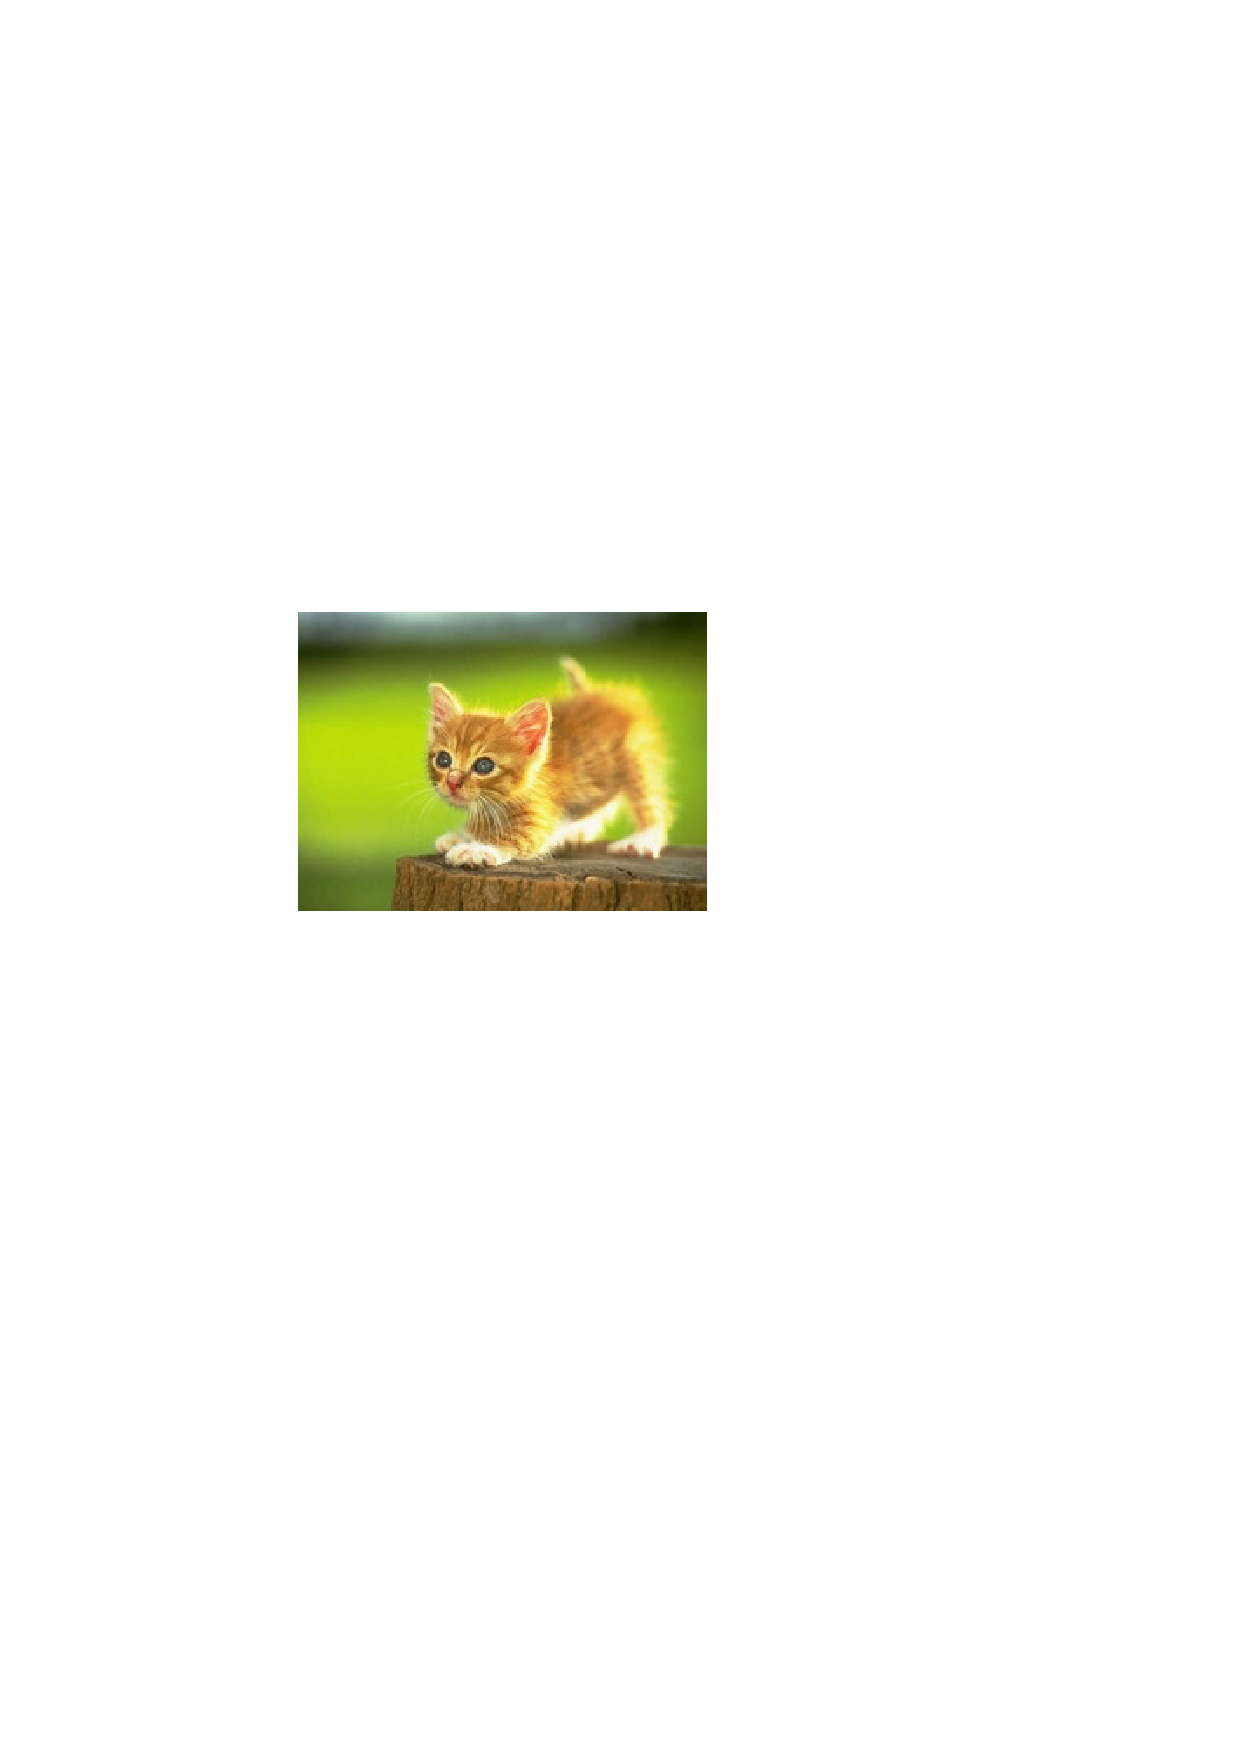
\includegraphics[width=.4\textwidth]{fig-example.pdf}
\caption{一个图片}\label{fig:1}
\end{figure}

\begin{figure}[!h]
\centering
  \begin{subfigure}[b]{0.3\textwidth}
  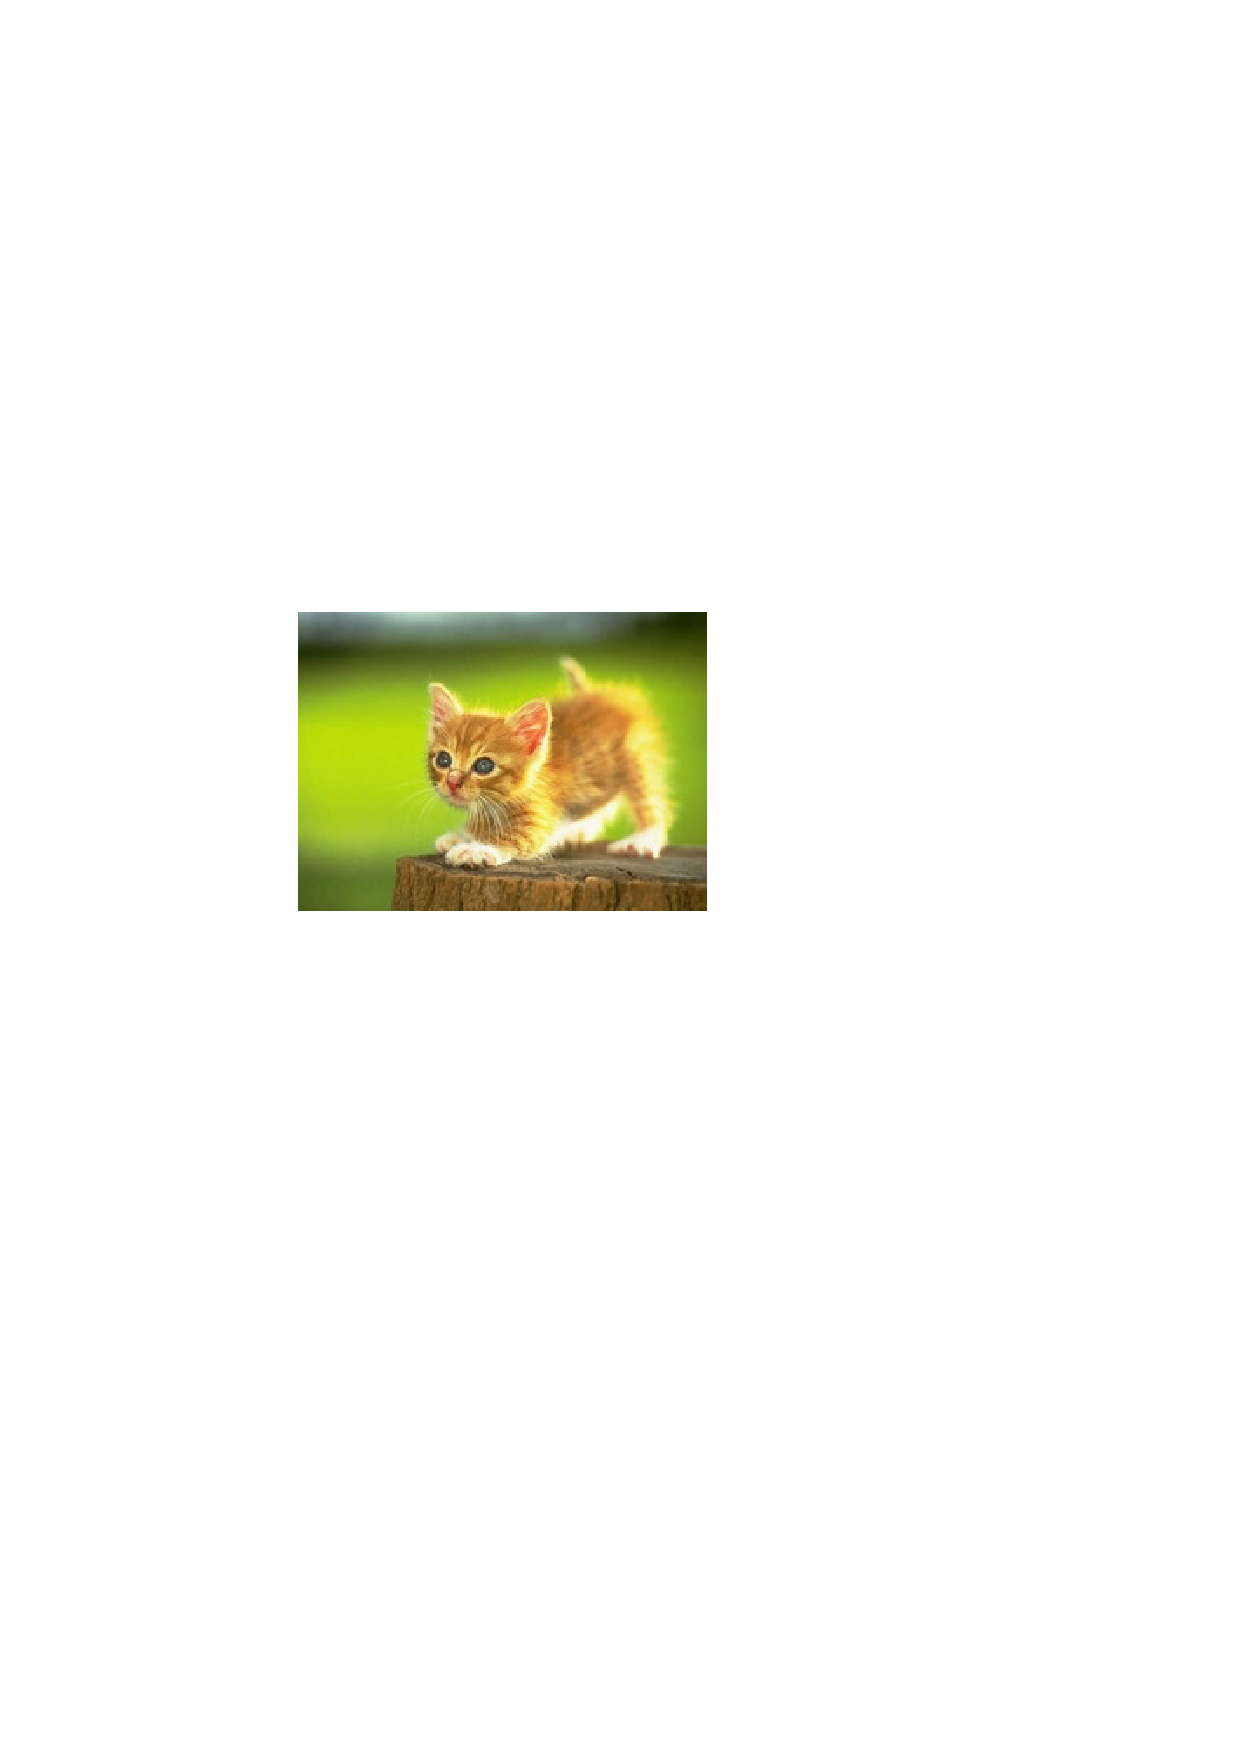
\includegraphics[width=\textwidth]{fig-example.pdf}
  \caption{图片1}\label{fig:2-1}
  \end{subfigure}
  ~
  \begin{subfigure}[b]{0.3\textwidth}
  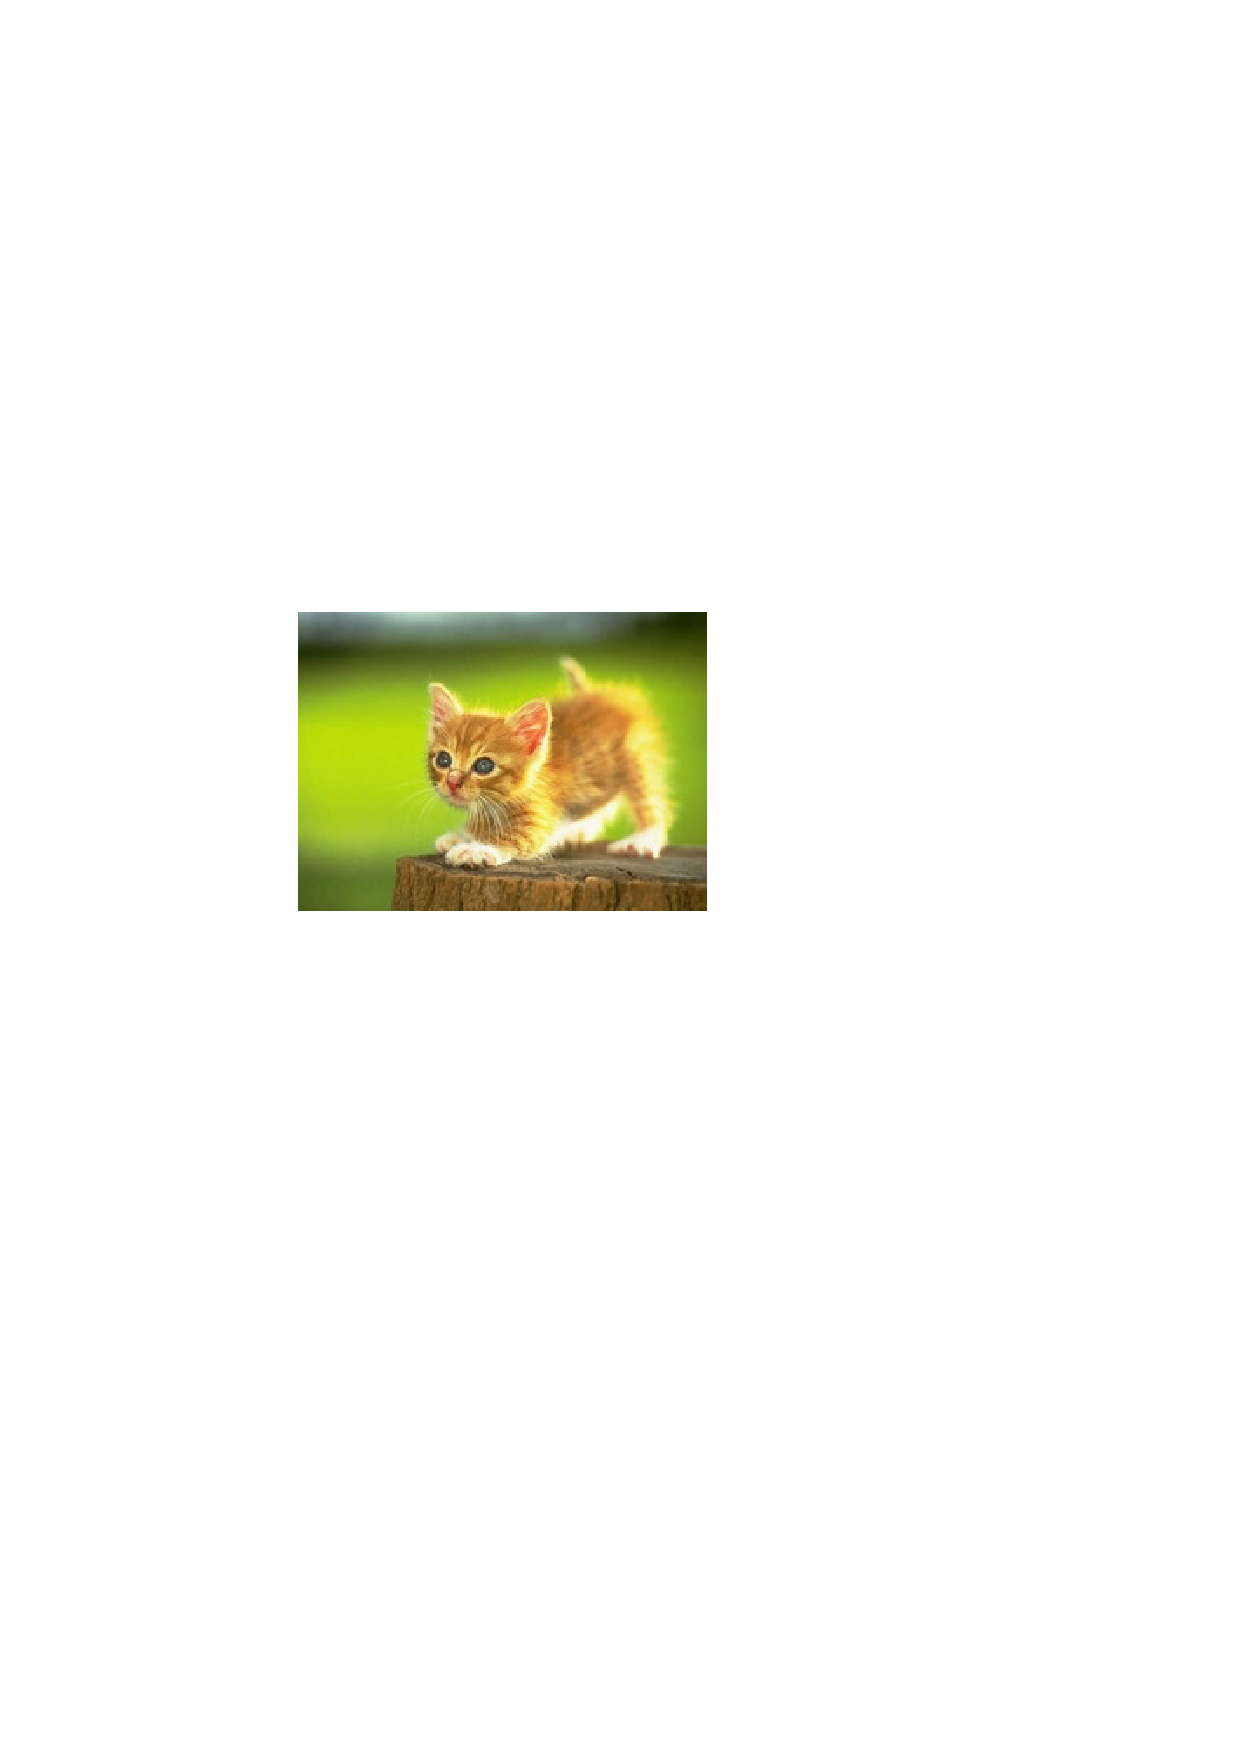
\includegraphics[width=\textwidth]{fig-example.pdf}
  \caption{图片2}\label{fig:2-2}
  \end{subfigure}
\caption{多个图片}\label{fig:2}
\end{figure}

\section{参考文献示例}
这是一篇中文参考文献\cite{TEXGURU99};这是一篇英文参考文献\cite{knuth};同时引用\cite{TEXGURU99,knuth}。

\section[\textbackslash{}autoref 测试]{\texttt{\textbackslash{}autoref} 测试}

\begin{description}
  \item[公式] \autoref{eq:1}
  \item[脚注] \autoref{footnote:1}
  \item[项] \autoref{item:1},\autoref{item:2},\autoref{item:3}
  \item[图] \autoref{fig:1}
  \item[表] \autoref{tab:1}
  \item[附录] \autoref{appendix:1}
  \item[章] \autoref{chapter:1}
  \item[小节] \autoref{sec:1},\autoref{sec:2},\autoref{sec:3}
  \item[算法] \autoref{alg:1},\autoref{alg_line:1}
  \item[证明环境] \autoref{def:1},\autoref{proposition:1},\autoref{axiom:1},\autoref{lemma:1},\autoref{theorem:1},\autoref{proof:1}
\end{description}


\backmatter
\bibliography{ref-example}
\appendix
\chapter{这是一个附录}\label{appendix:1}
附录正文。
\end{document}
%</example>
%<*example-bib>
@BOOK{TEXGURU99,
  AUTHOR        = "{\TeX}Guru",
  TITLE         = "{\LaTeXe} Manual",
  YEAR          = "1999"
}

@BOOK{knuth,
  AUTHOR        = "{Donald E. Knuth}",
  TITLE         = "The \TeX{}book",
  publisher     = "Addison–Wesley Pub. Co.",
  address       = "MA",
  YEAR          = "1984"
}
%</example-bib>
% \fi
\endinput
